%%%%%%%%%%%%%%%%%%%%%%%%%%%%%%%%%%%%%%%%%%%%%%%%%%%%%%%%%%%%%%%%%%%%%%%%%%
%
% Copyright (c) 2012 Jorge Nunes, All Rights Reserved.
%
%%%%%%%%%%%%%%%%%%%%%%%%%%%%%%%%%%%%%%%%%%%%%%%%%%%%%%%%%%%%%%%%%%%%%%%%%%

\documentclass[11pt]{article}

\usepackage[portuges]{babel}
\usepackage[utf8]{inputenc} 
\usepackage{a4}
\usepackage{amsfonts}
\usepackage{float}
\usepackage{graphicx}
\usepackage[colorlinks=true]{hyperref}
\usepackage{subfigure}






\title{$L$-Systems}
\author{Jorge Nunes ({\tt\href{mailto:jorgefranconunes@gmail.com}{jorgefranconunes@gmail.com}})}
\date{December 2012}





\begin{document}


\maketitle

\begin{abstract}
\noindent Some rumblings\ldots
\end{abstract}





\section{Koch island}

\begin{tabular}{ll}
Axiom: & $F - - F - - F$ \\
Production rules: & $F \to F + F - - F + F$ \\
& $+ \to +$ \\
& $- \to -$ \\
Turn angle $\delta$: & 60$^o$ \\
\end{tabular}


\begin{figure}[H]
  \centering

  \subfigure[]{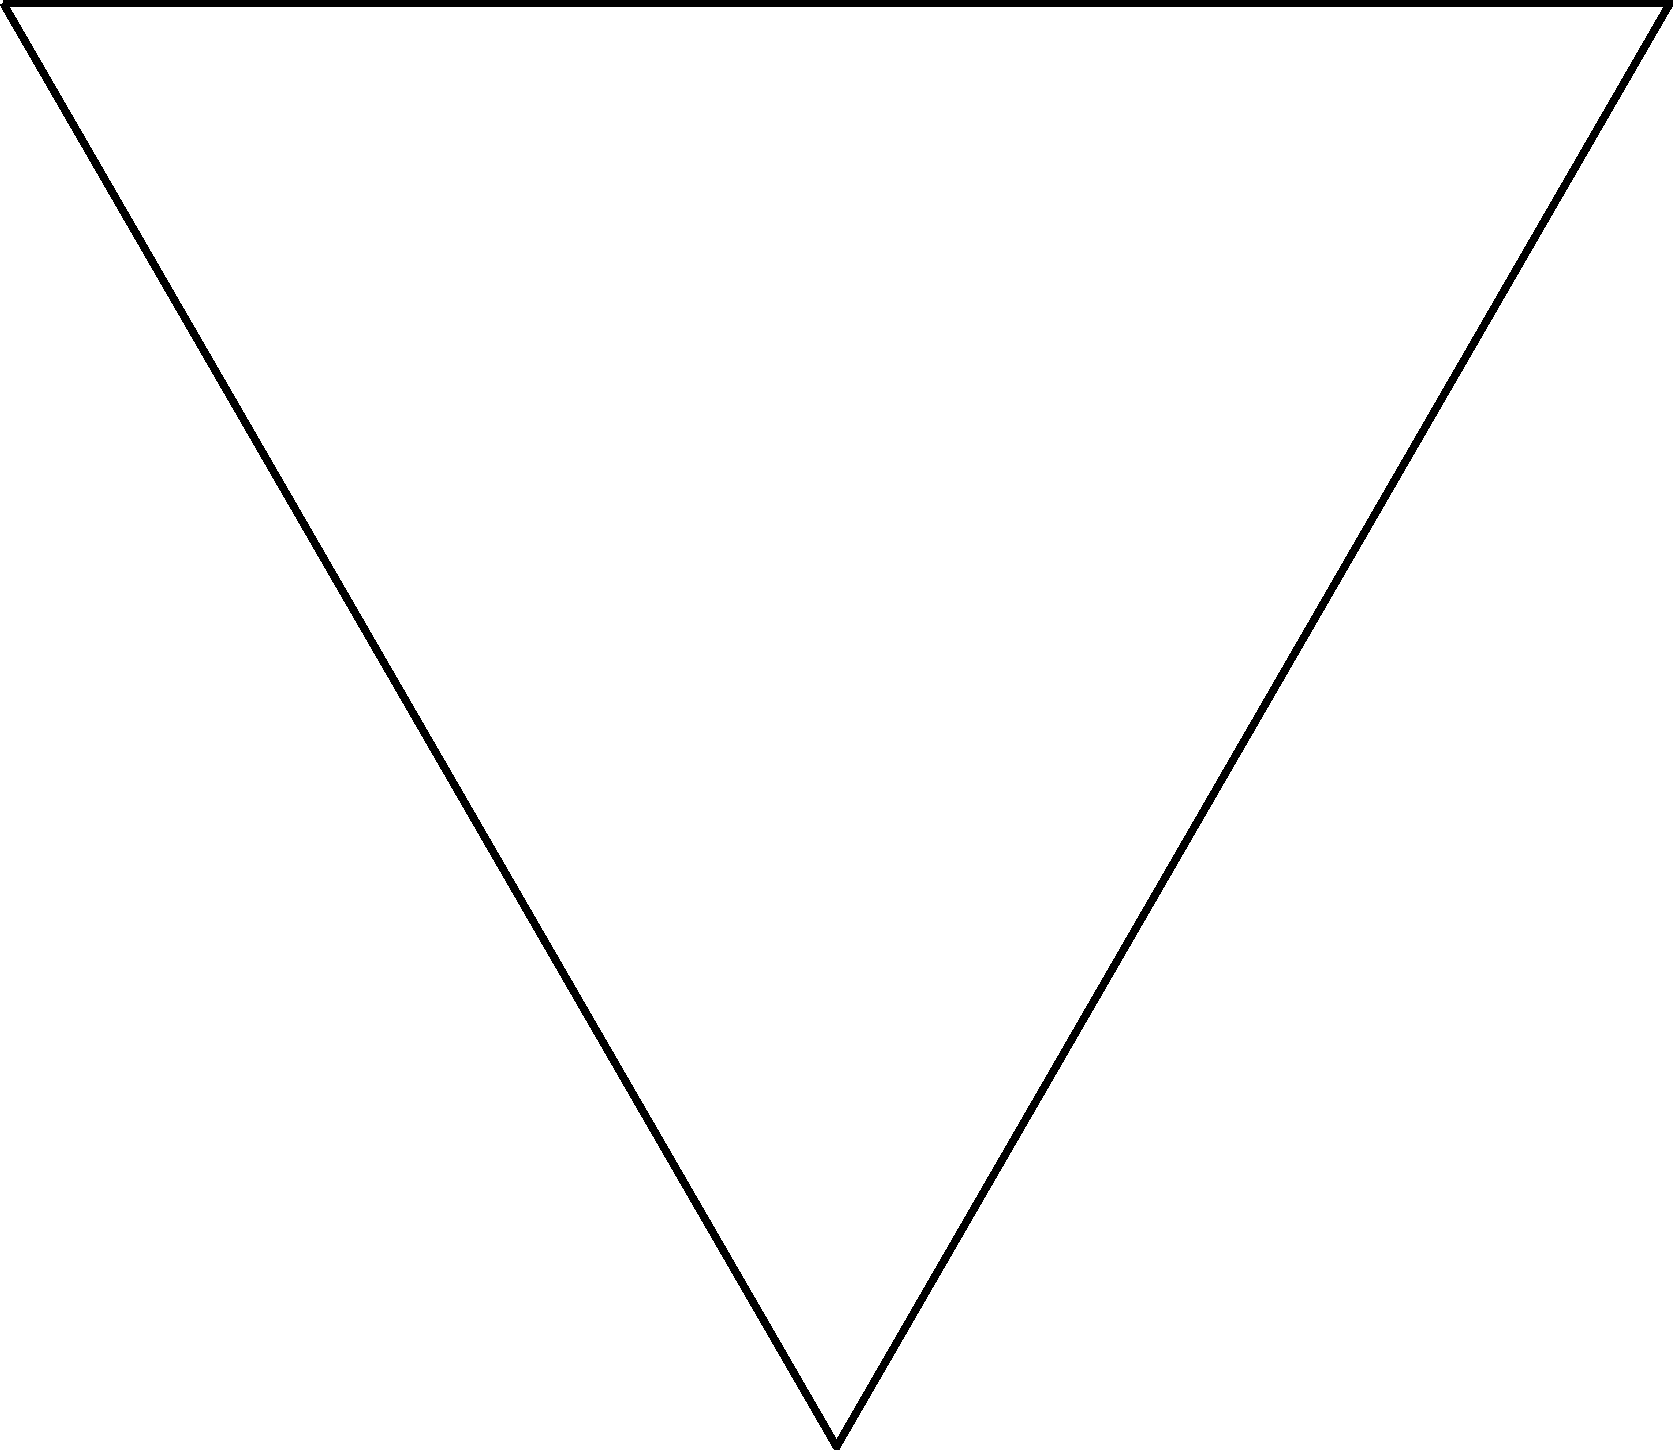
\includegraphics[width=0.3\textwidth]{../images/koch-island-00.pdf}}
  \hfill
  \subfigure[]{
\includegraphics[width=0.3\textwidth]{../images/koch-island-01.pdf}}
  \hfill
  \subfigure[]{
\includegraphics[width=0.3\textwidth]{../images/koch-island-02.pdf}}

  \subfigure[]{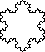
\includegraphics[width=0.3\textwidth]{../images/koch-island-03.pdf}}
  \hfill
  \subfigure[]{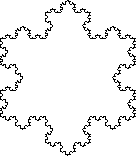
\includegraphics[width=0.3\textwidth]{../images/koch-island-04.pdf}}
  \hfill
  \subfigure[]{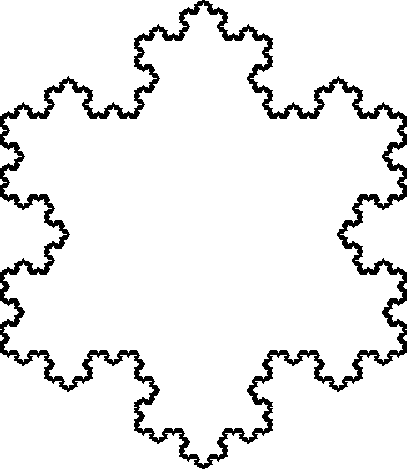
\includegraphics[width=0.3\textwidth]{../images/koch-island-05.pdf}}

  \caption{The axiom and the first five iterations of the Koch island curve.}
\end{figure}





\section{Quadratic Koch island}

\begin{tabular}{ll}
Axiom: & $F + F + F + F$ \\
Production rules: & $F \to F + F - F - F F + F + F - F$ \\
& $+ \to +$ \\
& $- \to -$ \\
Turn angle $\delta$: & 90$^o$ \\
\end{tabular}


\begin{figure}[H]
  \centering

  \subfigure[]{
\includegraphics[width=0.3\textwidth]{../images/koch-quadratic-00.pdf}}
  \hfill
  \subfigure[]{
\includegraphics[width=0.3\textwidth]{../images/koch-quadratic-01.pdf}}
  \hfill
  \subfigure[]{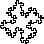
\includegraphics[width=0.3\textwidth]{../images/koch-quadratic-02.pdf}}

  \subfigure[]{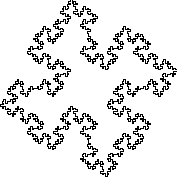
\includegraphics[width=0.3\textwidth]{../images/koch-quadratic-03.pdf}}
  \hfill
  \subfigure[]{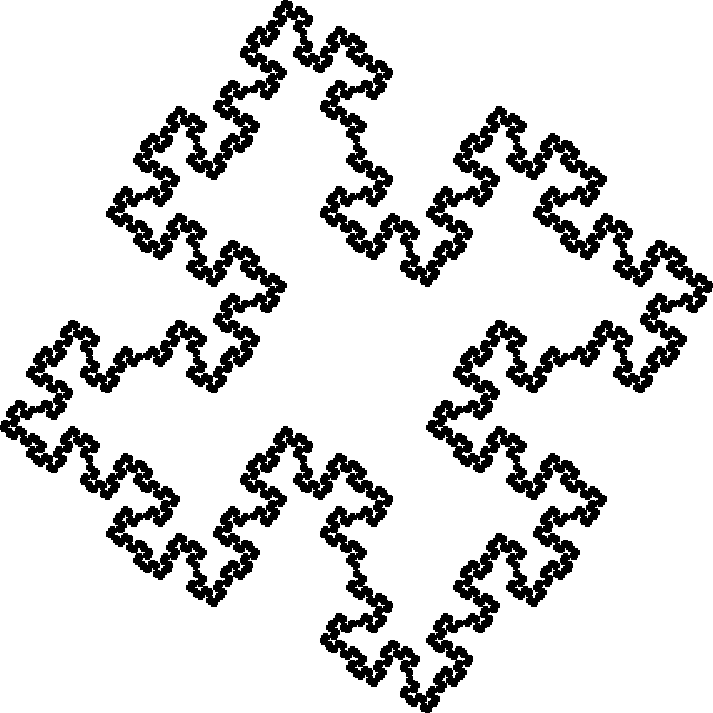
\includegraphics[width=0.3\textwidth]{../images/koch-quadratic-04.pdf}}
  \hfill
  \subfigure[]{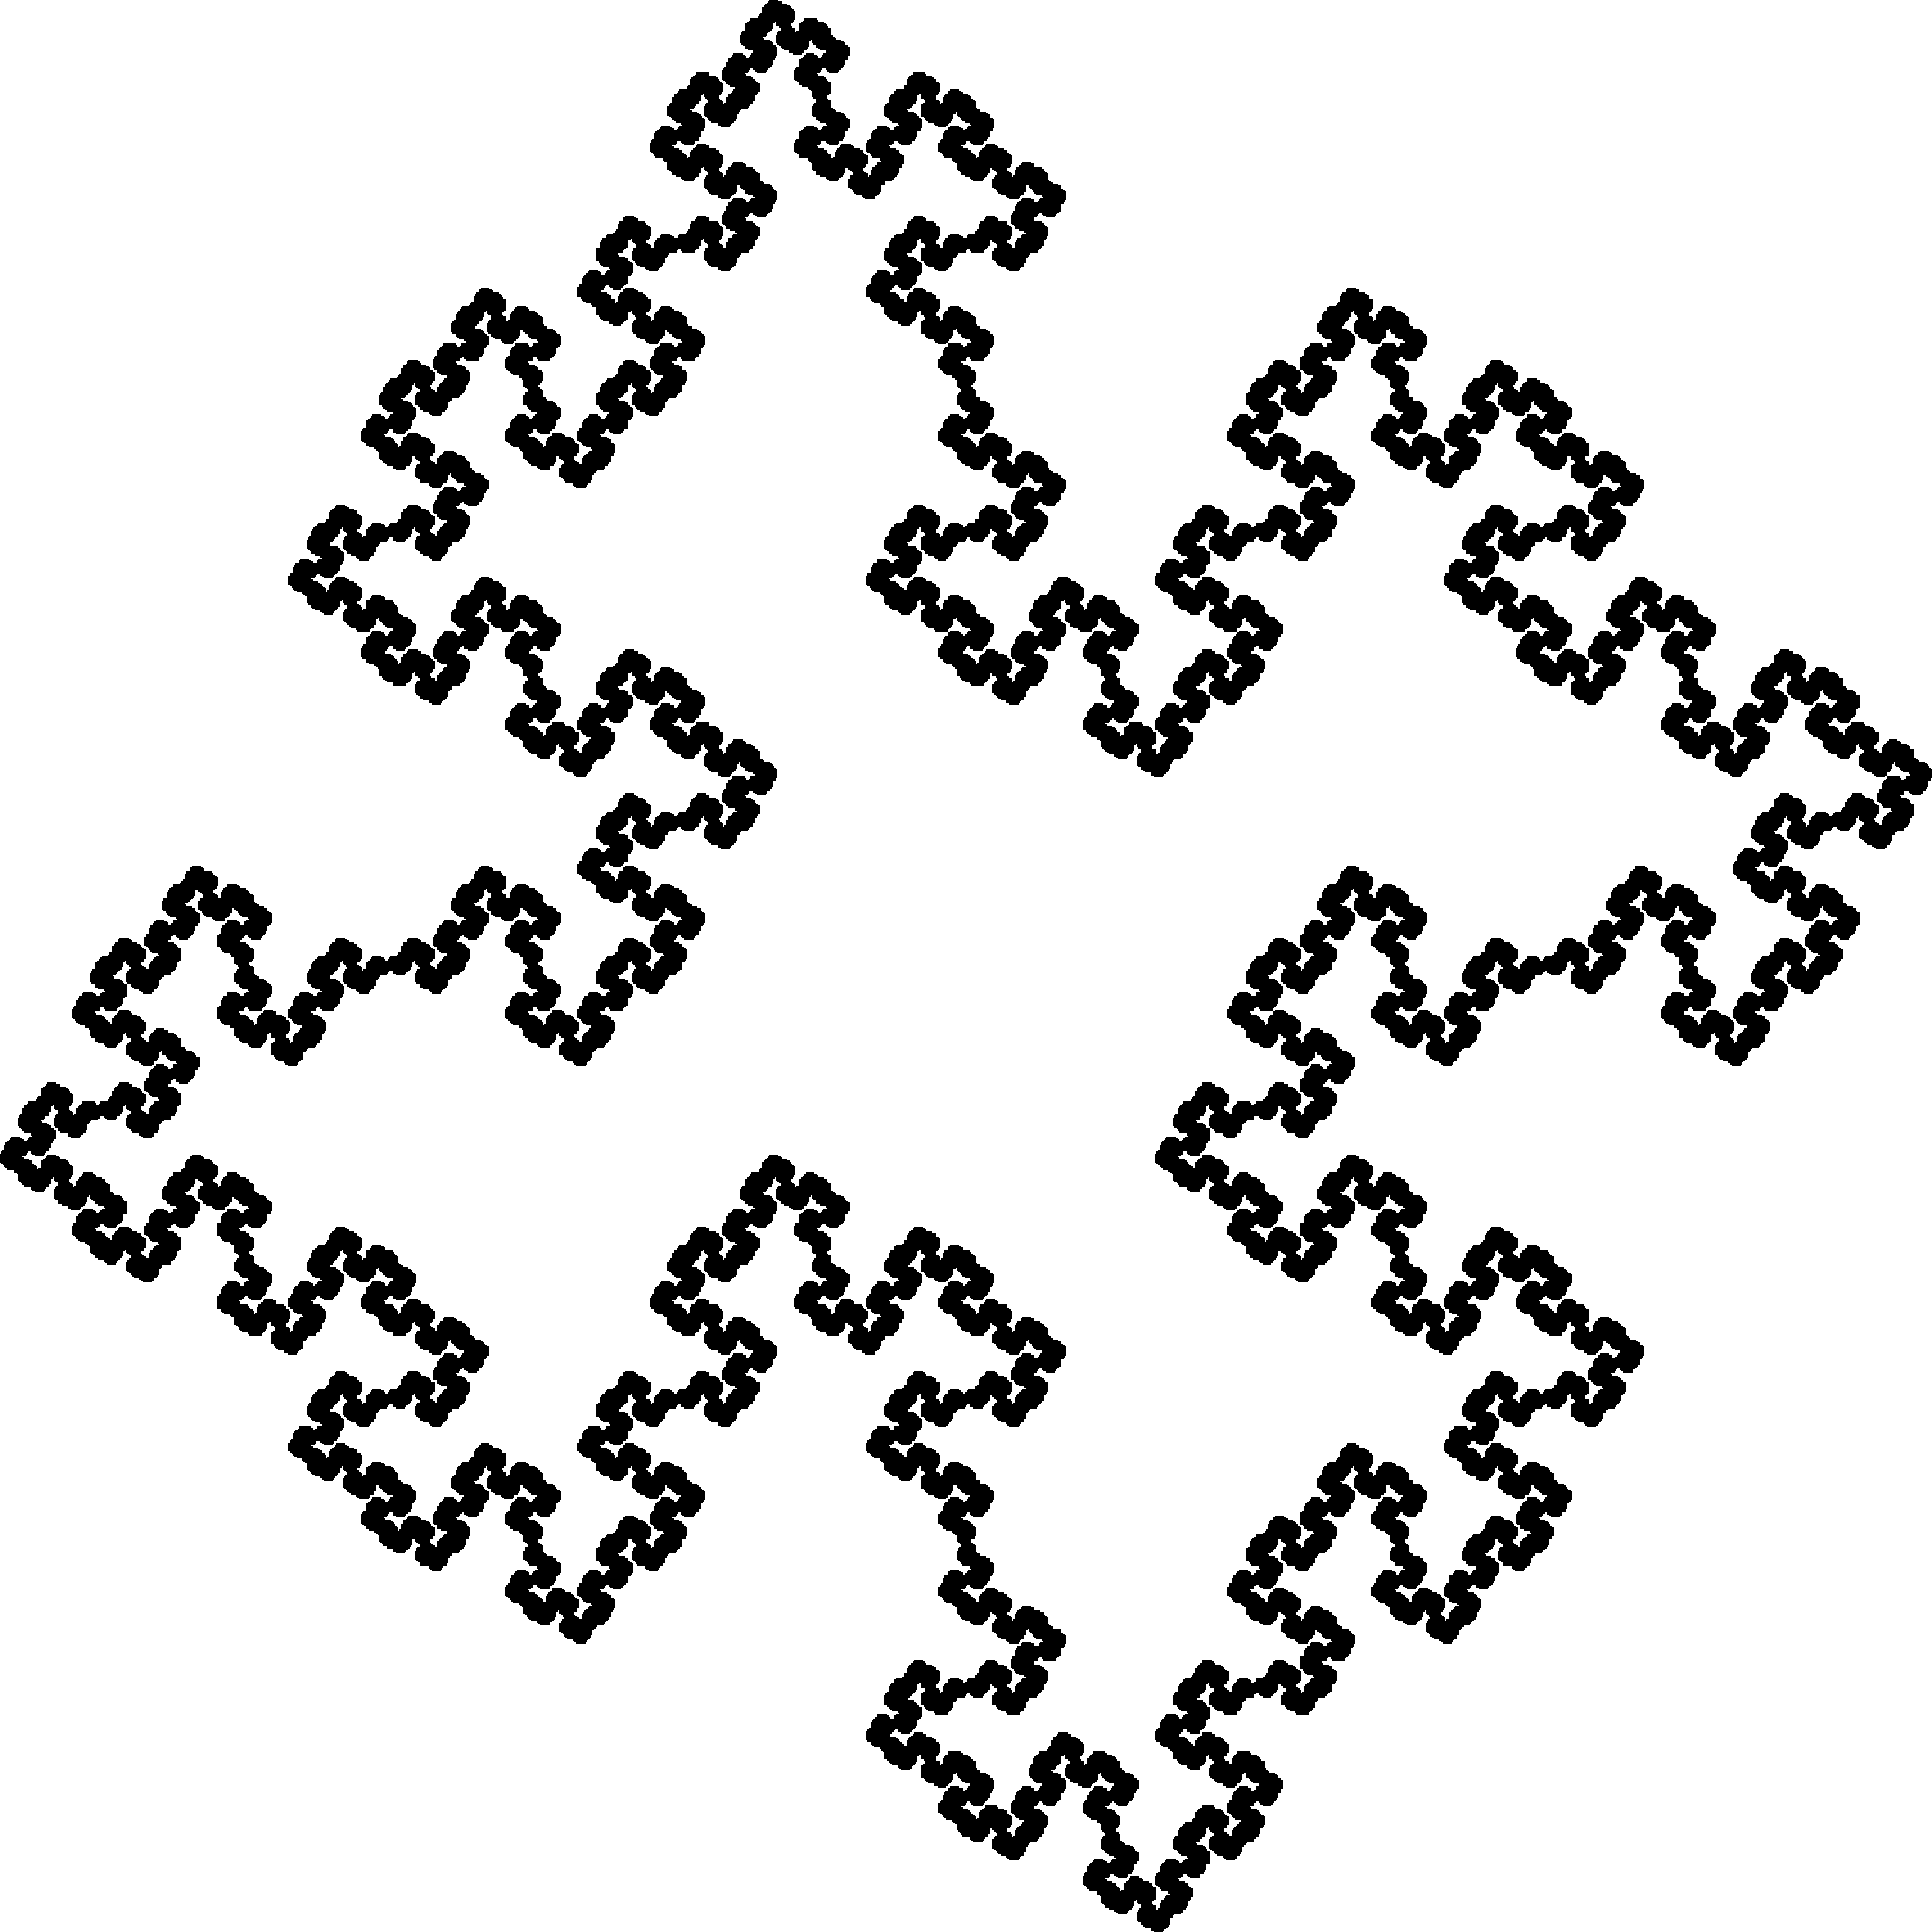
\includegraphics[width=0.3\textwidth]{../images/koch-quadratic-05.pdf}}

  \caption{The axiom and the first five iterations of the quadratic
    Koch island.}
\end{figure}





\section{Sierpinski arrowhead}

\begin{tabular}{ll}
Axiom: & $L$ \\
Production rules: & $L \to + R - L - R +$ \\
& $R \to - L + R + L - $ \\
& $+ \to +$ \\
& $- \to -$ \\
Turn angle $\delta$: & 60$^o$ \\
\end{tabular}

\begin{figure}[H]
  \centering

  \subfigure[]{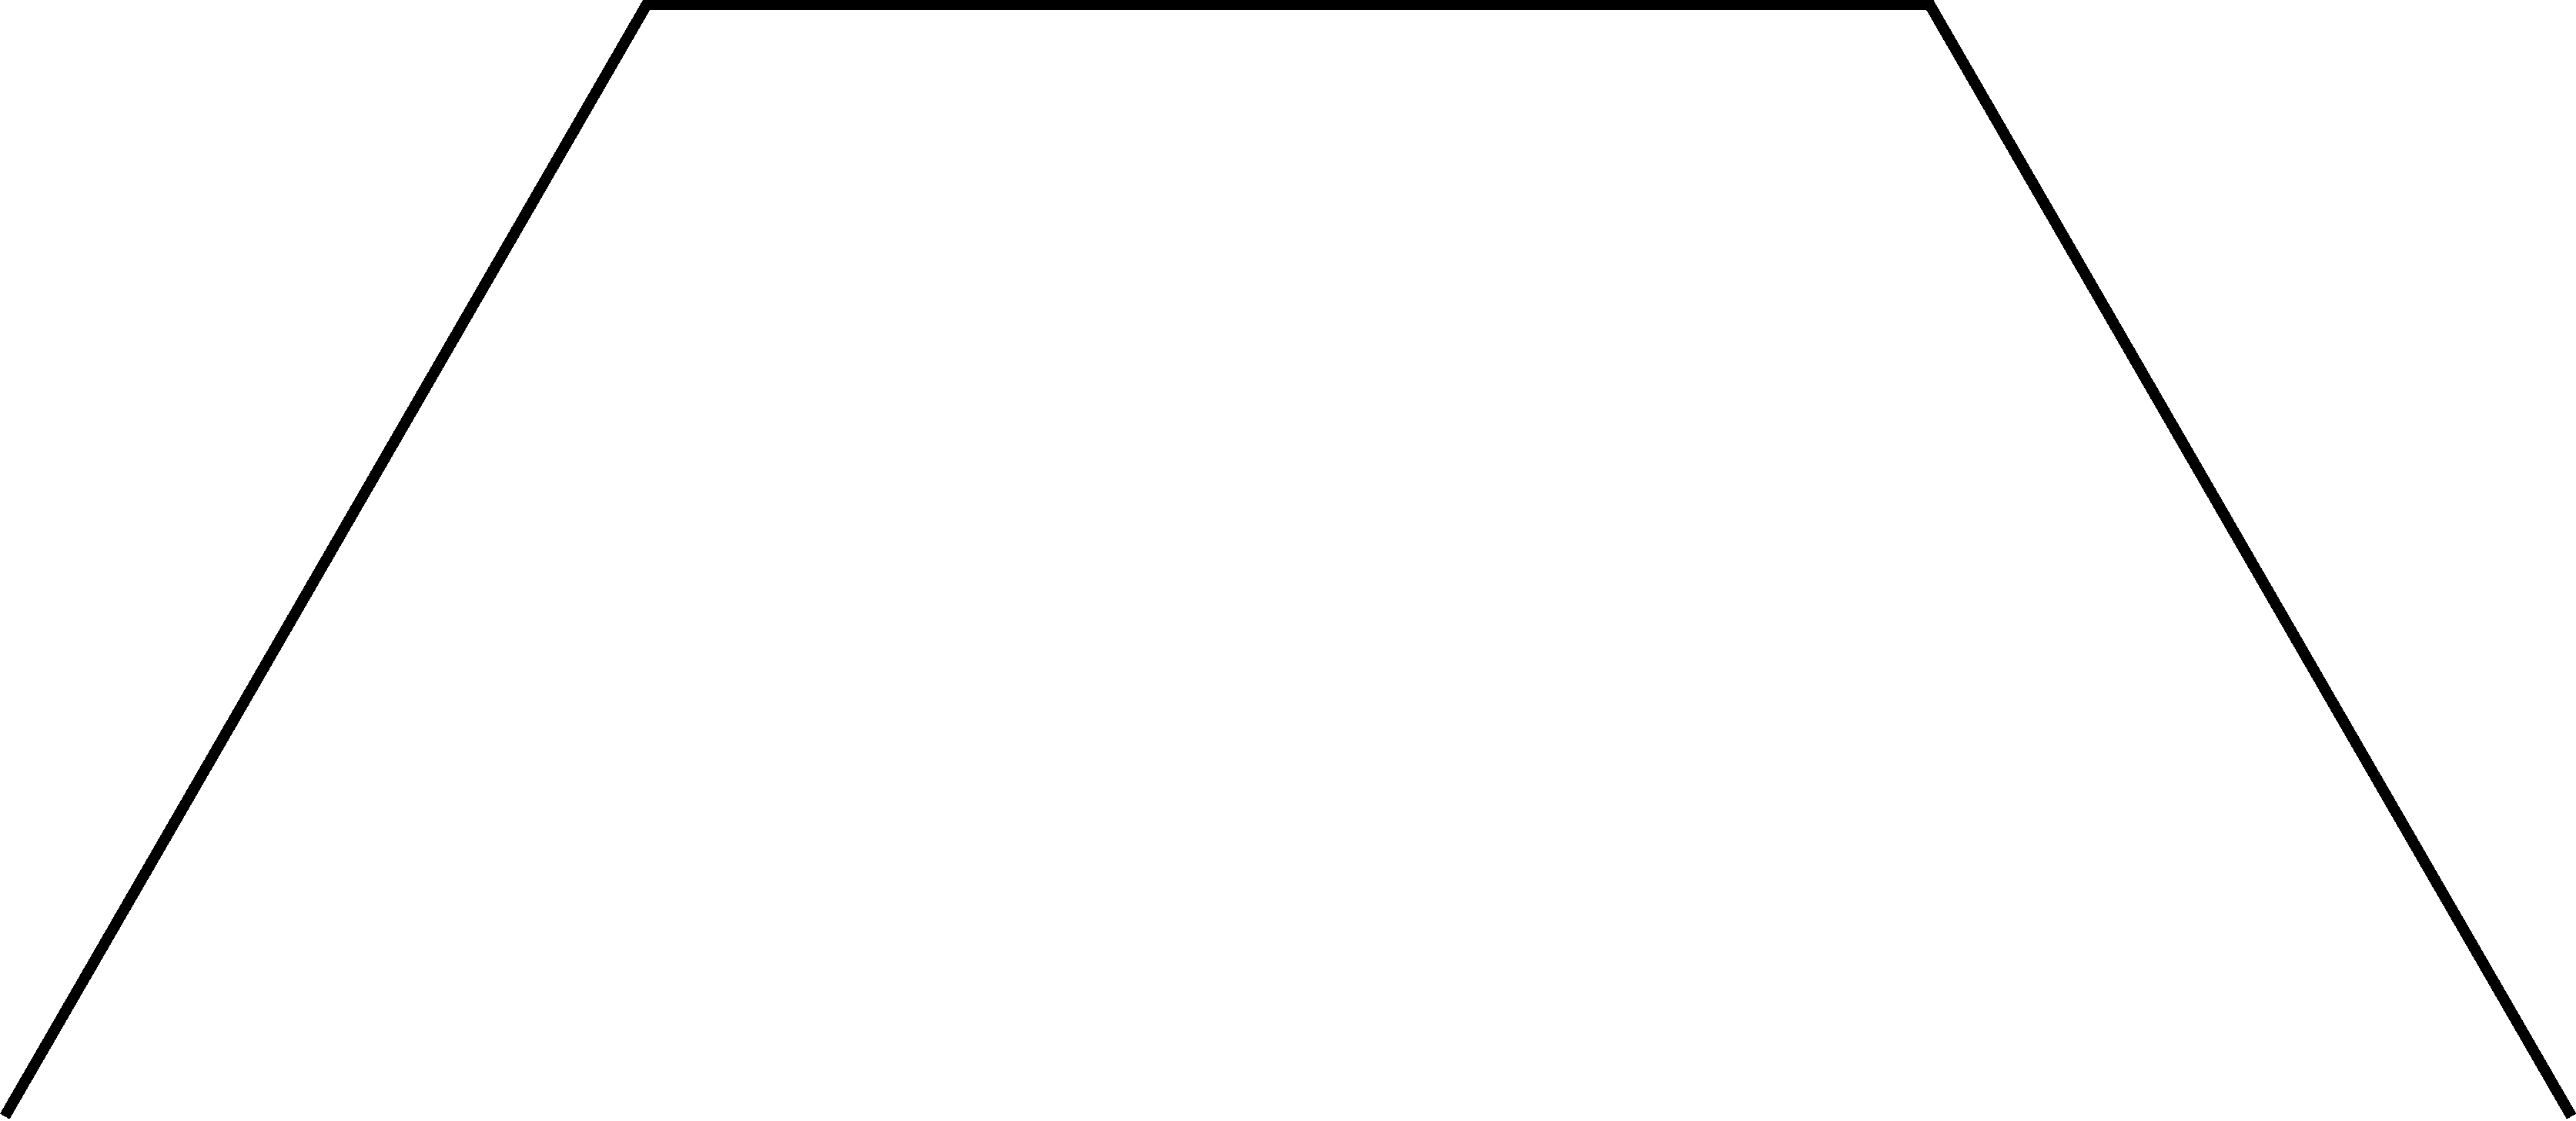
\includegraphics[width=0.3\textwidth]{../images/sierpinski-00.pdf}}
  \hfill
  \subfigure[]{
\includegraphics[width=0.3\textwidth]{../images/sierpinski-01.pdf}}
  \hfill
  \subfigure[]{
\includegraphics[width=0.3\textwidth]{../images/sierpinski-02.pdf}}

  \subfigure[]{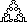
\includegraphics[width=0.3\textwidth]{../images/sierpinski-03.pdf}}
  \hfill
  \subfigure[]{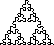
\includegraphics[width=0.3\textwidth]{../images/sierpinski-04.pdf}}
  \hfill
  \subfigure[]{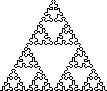
\includegraphics[width=0.3\textwidth]{../images/sierpinski-05.pdf}}

  \caption{The axiom and the first five iterations of the Sierpinski arrowhead.}
\end{figure}





\section{Hilbert curve}

\begin{tabular}{ll}
Axiom: & $L$ \\
Production rules: & $F \to F$ \\
& $L \to + R F - L F L - F R +$ \\
& $R \to - L F + R F R + F L -$ \\
& $+ \to +$ \\
& $- \to -$ \\
Turn angle $\delta$: & 90$^o$ \\
\end{tabular}


\begin{figure}[H]
  \centering

  \subfigure[]{
\includegraphics[width=0.3\textwidth]{../images/hilbert-00.pdf}}
  \hfill
  \subfigure[]{
\includegraphics[width=0.3\textwidth]{../images/hilbert-01.pdf}}
  \hfill
  \subfigure[]{
\includegraphics[width=0.3\textwidth]{../images/hilbert-02.pdf}}

  \subfigure[]{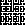
\includegraphics[width=0.3\textwidth]{../images/hilbert-03.pdf}}
  \hfill
  \subfigure[]{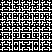
\includegraphics[width=0.3\textwidth]{../images/hilbert-04.pdf}}
  \hfill
  \subfigure[]{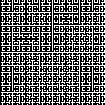
\includegraphics[width=0.3\textwidth]{../images/hilbert-05.pdf}}

  \caption{The axiom and the first five iterations of the Hilbert curve.}
\end{figure}





\section{Dragon curve}

\begin{tabular}{ll}
Axiom: & $D$ \\
Production rules: & $D \to - D + + E$ \\
& $E \to D - - E +$ \\
& $+ \to +$ \\
& $- \to -$ \\
Turn angle $\delta$: & 45$^o$ \\
\end{tabular}

\begin{figure}[H]
  \centering

  \subfigure[]{
\includegraphics[width=0.3\textwidth]{../images/dragon-00.pdf}}
  \hfill
  \subfigure[]{
\includegraphics[width=0.3\textwidth]{../images/dragon-01.pdf}}
  \hfill
  \subfigure[]{
\includegraphics[width=0.3\textwidth]{../images/dragon-02.pdf}}

  \subfigure[]{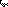
\includegraphics[width=0.3\textwidth]{../images/dragon-03.pdf}}
  \hfill
  \subfigure[]{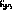
\includegraphics[width=0.3\textwidth]{../images/dragon-04.pdf}}
  \hfill
  \subfigure[]{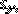
\includegraphics[width=0.3\textwidth]{../images/dragon-05.pdf}}

  \subfigure[]{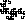
\includegraphics[width=0.3\textwidth]{../images/dragon-06.pdf}}
  \hfill
  \subfigure[]{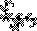
\includegraphics[width=0.3\textwidth]{../images/dragon-07.pdf}}
  \hfill
  \subfigure[]{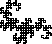
\includegraphics[width=0.3\textwidth]{../images/dragon-08.pdf}}

  \subfigure[]{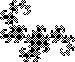
\includegraphics[width=0.3\textwidth]{../images/dragon-09.pdf}}
  \hfill
  \subfigure[]{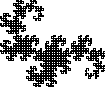
\includegraphics[width=0.3\textwidth]{../images/dragon-10.pdf}}
  \hfill
  \subfigure[]{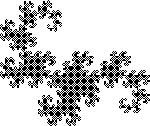
\includegraphics[width=0.3\textwidth]{../images/dragon-11.pdf}}

  \caption{The axiom and the first eleven iterations of the dragon
    curve.}
\end{figure}

  



\end{document}

